\section{Boundary Equation Derivation}
\subsection{Proposing the Problem}
The term ``Electrowetting" refers to distinct scenarios, such as the two cases in Figure \ref{fig:ew_2cases}. This chapter addresses a charged droplet on an electrically negligible substrate, surrounded by air.
\begin{figure}[H]
    \centering
\adjustbox{frame=0.25pt,frame,margin=0.1pt,color=mycolor}{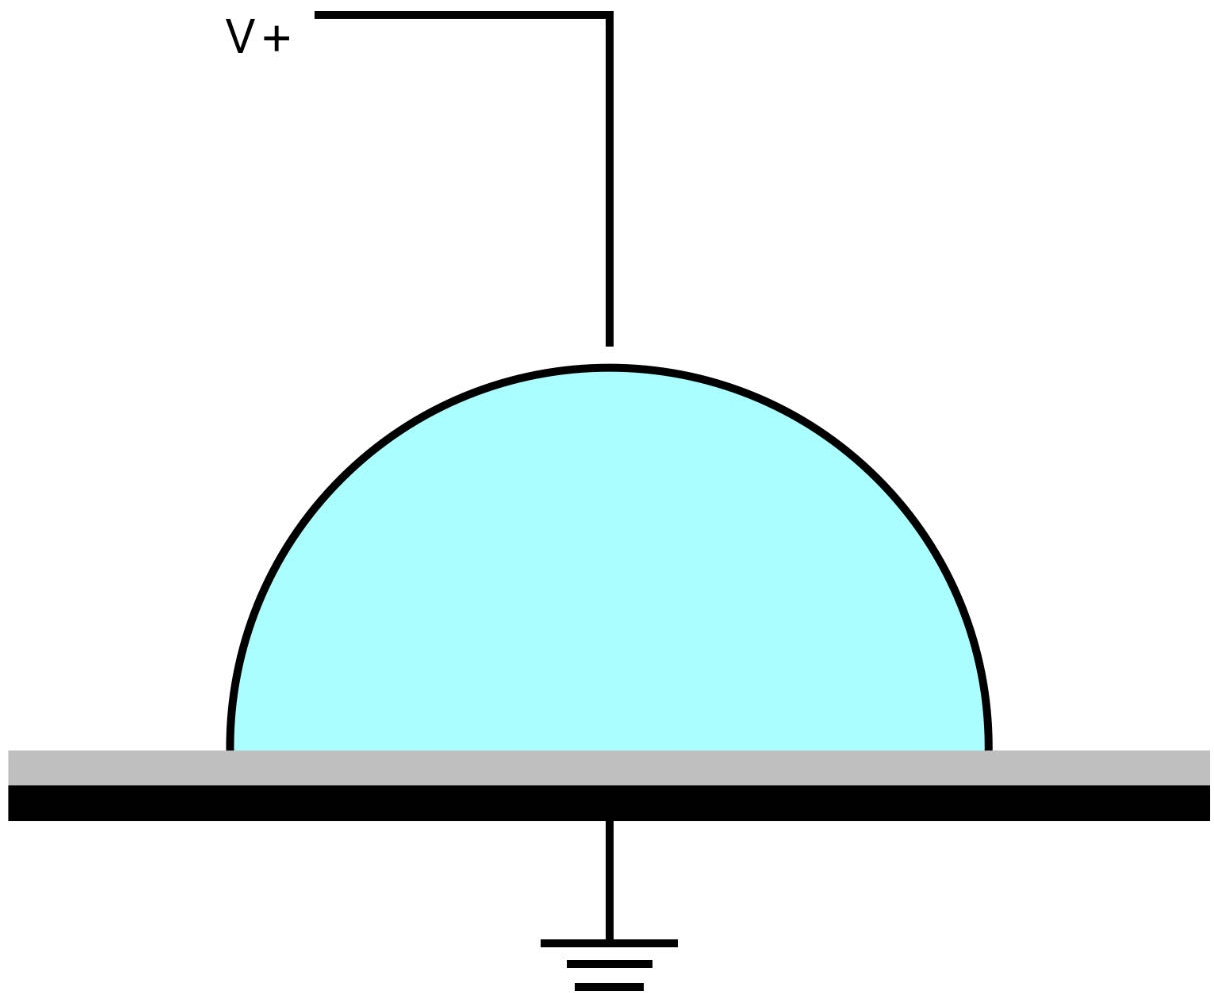
\includegraphics[width=0.405\linewidth]{Figs/sketch eletrode.jpg}}\hspace{.5em}
    \adjustbox{frame=0.25pt,frame,margin=0.1pt,color=mycolor}{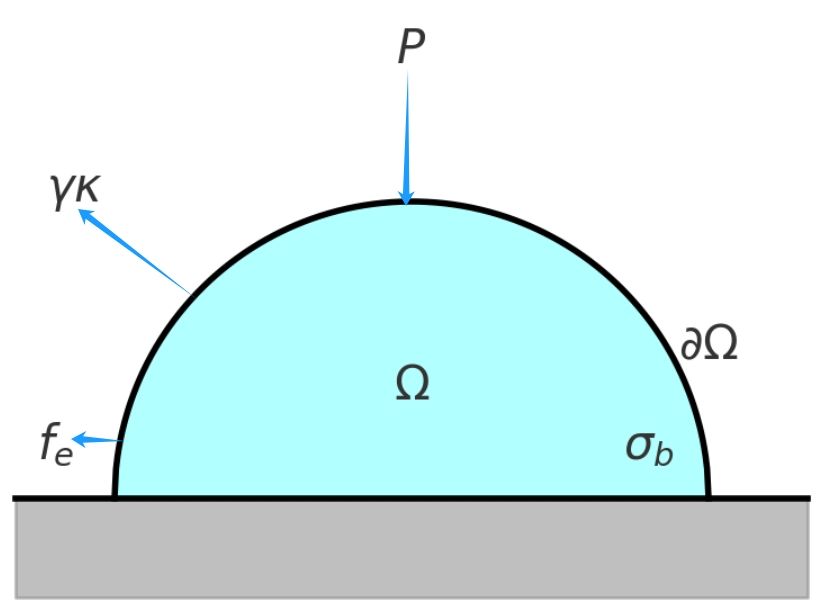
\includegraphics[width=0.445\linewidth]{Figs/setup, tension and force.png}} % Side by side images
    
    \caption{\small In the left figure, an electrode generates a voltage difference $V_+$ between the uncharged droplet and the conductor beneath an insulating layer. Meanwhile, the charged droplet with surface charge density $\sigma_b$ sits on an electrically negligible layer in the right figure. $\Omega\in\mathbb{R}^2$ represents the volume/area of the charged droplet. The balance between surface tension $\gamma\kappa$, pressure $P$, and the electric force $\vec{f}_e$—which is always a repulsive force—affects the droplet's shape $\partial \Omega$, while its volume $\Omega$ remains unchanged. The directions of $\gamma\kappa$ and $P$ depend on the specific conditions.
}
     \label{fig:ew_2cases}
\end{figure}
\noindent The conducting fluid droplet occupies $\Omega\in\mathbb{R}^2$ , the charge generates an electric field $\vec{E}$, together with the mechanical energy $\gamma\mathcal{P}$ from surface tension, the energy equation, which can date back to \citet{Rayleigh_1882}, is
\begin{equation}\label{eqn:minE}
    \mathcal{E} = \gamma \mathcal{P} - \frac{\epsilon_0 \epsilon_r}{2} \int_{R^2 \setminus \Omega} |E|^2 \, dS
\end{equation}

The electric energy $\mathcal{E}_e$ is the second term on the right of equation (\ref{eqn:minE}). The integral area ${\mathbb{R}^2 \setminus \Omega}$ implies that there is no electric field inside the droplet. $\epsilon_0 \epsilon_r$ is the permittivity, $\gamma$ is the surface tension, $\mathcal{P}$ is the length of the liquid-vapour interface, as defined in \citet{Crowdy2015}, equation (1).  The boundary equation on the liquid-vapour interface, from equation (\ref{eqn:minE}), is
\vspace{-0.5em}\begin{equation}\label{eqn:FonB}
\gamma \kappa - \frac{\sigma^2}{2 \epsilon_0 \epsilon_r} = -p\vspace{-0.5em}
\end{equation}
\subsection{Forces at the Stationary Boundary}
\hspace{0em}\indent \citet{Crowdy2015} proposed Equation (\ref{eqn:FonB}) by the variation of energy. Here, we first derive the equation (\ref{eqn:FonB}) from the forces on the droplet curve $\partial \Omega$. At any point on the droplet curve, let $\hat{n}$ be the normal direction pointing outward of the curve. The pressure difference $p\hat{n}$ and the surface tension, $\gamma \kappa \df l\hat{n} $, will be balanced by the electric force\footnote{Refer to equation (2.50), \citet{Griffiths_2017}, page 103.}
%\vspace{-0.5em}
\[
\vec{f}_e=\frac{\sigma}{2} (\vec{E}_{above}+\vec{E}_{below})%\vspace{-0.5em}
\]
The interior area of the conductor droplet is an equipotential area hence $\vec{E}_{below}\equiv0$, whereas  
%\vspace{-0.5em}
\[
\vec{E}_{above}|_{\partial \Omega}=-\nabla V|_{\partial \Omega}=-\left.\frac{\partial V}{\partial n}\hat{n}\right|_{\partial\Omega}%\vspace{-0.5em}
\]
$\vec{E}$ is caused by the surface charge density $\sigma$. According to equation (\ref{eqn:ed.line}) and equation (\ref{eqn:f.line}), the electrostatic pressure along the curve, is
%\vspace{-0.5em}
\[p_e=\frac{\sigma}{2}\left|\vec{E}_{above}\right|=-\frac{\sigma}{2}\frac{\partial V}{\partial n}=+\frac{\sigma^2}{2\epsilon_0\epsilon_r}%\vspace{-0.5em}
\]
This found the same result as in \citet{Fontelos2008}, equation (4). The force along $\hat{n}$ is:%\vspace{-0.75em}
\[0=\gamma\kappa\hat{n}+p\hat{n}+\frac{1}{2}\sigma \vec{E}%\vspace{-0.75em}
\]
In the stabilised circumstance, a charged conducting droplet has balanced electric force, pressure, and surface tension perpendicularly along its boundary line.
\subsection{Derivation Using the Divergence Theorem}
\hspace{0em}\indent We next try the divergence theorem. The variation in the electric field $\delta E_e$ is:
\begin{equation*}
    \delta \mathcal{E}_e=+\delta\left(-\frac{\epsilon}{2}\int_{\mathbb{R}^2\setminus\Omega}|E|^2 \df S
\right)=\int_{\delta\partial\Omega}...-\frac{\epsilon}{2}\int_{\mathbb{R}^2\setminus\Omega}\delta|E|^2 \df S\simeq-\frac{\epsilon}{2}\int_{\mathbb{R}^2\setminus\Omega}2\vec{E}\cdot\delta\vec{E} \df S
\end{equation*}
Let $\vec{G}\coloneqq\vec{E}\delta V$, $V$ is the voltage.
\begin{equation*}
    \begin{split}
    \delta \mathcal{E}_e&=-\epsilon\int_{\mathbb{R}^2\setminus\Omega}\vec{E}\cdot\delta(-\nabla V) \df S=\epsilon\int_{\mathbb{R}^2\setminus\Omega}\vec{E}\cdot(\nabla \delta V) \df S
    \end{split}
    \end{equation*}
Use $\nabla\cdot(\vec{A}\phi)=\phi\nabla\cdot\vec{A}+\vec{A}\cdot\nabla\phi$
\begin{equation}\label{eqn:div_find_0}
    \begin{split}
    \delta \mathcal{E}_e&=\epsilon\int_{\mathbb{R}^2\setminus\Omega}\nabla\cdot(\vec{E}\, \delta V) -\delta V \eqnmarkbox[black]{node1}{\nabla\cdot\vec{E}}\df S\\
    &=\epsilon\int_{\mathbb{R}^2\setminus\Omega}\nabla\cdot(\vec{E}\, \delta V) \df S \xlongequal[ ]{\text{div thm}}\oint_{...}\vec{G}\cdot\hat{n}\df l \epsilon=\int_{\partial \Omega}...+\eqnmarkbox[black]{node2}{\int_{r\rightarrow\infty}\vec{E}}\cdot\hat{n}\, \delta V\df l\\
    &=\epsilon\int_{\partial\Omega}\vec{E}\cdot\hat{n}\, \delta V \df l=\sigma\int_{\partial \Omega}\delta V \df l\\
    \end{split}
\end{equation}
\annotate[yshift=1em]{above, right, label above}{node1}{$\nabla \cdot \vec{E}|_{\mathbb{R}^2\setminus \Omega}= 0$}
\annotate[yshift=1em]{above, right, label above}{node2}{$=0,\vec{E}|_{r\rightarrow\infty}\rightarrow 0$}

\vspace{-1em}
\noindent Equation (\ref{eqn:ed.line}) shows $\vec{E}|_{\partial \Omega}=\sigma/\epsilon\hat{n}$. To have the desired result, we expect
\[\int_{\partial \Omega} \delta V \df l =-\frac{\sigma}{2\epsilon}\int_{\delta \partial \Omega}\df l\Longrightarrow\delta V = -\frac{\sigma}{2\epsilon}\delta l\]
Moreover\footnote{Refer to \cite{Griffiths_2017}, equation (2.50).}, \vspace{0.5em}
\[\delta V =  -\frac{1}{2}(\vec{E}_{above}+\eqnmarkbox[black]{node1}{{\vec{E}_{below}}})\cdot \delta \vec{l}=-\frac{\vec{E}_{above}}{2}\delta \vec{l}=-\frac{\sigma}{2\epsilon}\hat{n}\cdot \delta \vec{l}\]
\annotate[yshift=1.0em]{above, right, label above}{node1}{$=0$}

\vspace{-1.5em}
\noindent Since $V=\int \vec{E}\Longrightarrow \delta V \sim \vec{E}_{average}\cdot\delta\vec{d}$. Let $\delta l=\hat{n}\cdot\delta\vec{l}$, We derive the wanted equation,

\subsection{Variation of Minimal Energy Equation}
\label{Min_Eng}
\hspace{0em}\indent We lastly attempt the variation method. For energy minimization, a variation of the droplet curve $\delta\Omega$ leads to no change in energy, $\delta\mathcal{E}=0$. The corresponding variation in the surface tension and mechanical energy is:
\vspace{-0.5em}
\[\delta (\gamma\mathcal{P})=\gamma\delta\mathcal{P}\hspace{0.5em},\hspace{1em}\delta\mathcal{P}=\int_{\partial \delta\Omega}\kappa\df l\vspace{-0.5em}\]

Furthermore, since all the charges are distributed on the boundary $\partial \Omega$, assume\footnote{for a point charge, $E\sim r^{-2}\Longrightarrow\int E \sim O(r^{-1})$.} $\mathcal{E}_e|_{r\rightarrow\infty}\leq O(r^{-1})\sim 0$. Known $\mathcal{E}_e|_{\partial \Omega}=\sigma/\epsilon$ from equation (\ref{eqn:ed.line}), where $\sigma$ is the line charge density,
\[
\mathcal{E}_e=-\frac{\epsilon}{2}\int_{\mathbb{R}^2\setminus \Omega}|E|^2\df S=-\frac{\epsilon}{2}\int_{\partial \Omega}|\frac{\sigma}{\epsilon}|^2\df l+ \text{others} \Longrightarrow\delta \mathcal{E}_e \approx-\frac{\sigma^2}{2\epsilon}\int_{\partial \delta\Omega}\df l+\delta\, \text{others}
\]
Presume that a small variation of the boundary curve has a negligible effect in the region other than $\partial \Omega$, hence $\delta\, \text{others}\equiv0$, which is hinted in equation (\ref{eqn:div_find_0}). Sum up the two parts gives
\vspace{-0.5em}\[
\gamma \int_{\partial \Omega} \kappa \df l - \frac{\sigma^2}{2\epsilon}\int_{\partial \Omega}=0\vspace{-0.5em}
\]
Together with equation (\ref{Delta_P}), $\Delta p = \gamma \kappa$, the surface tension and pressure balance each other in the absence of electric force, we achieve the wanted formula.
\subsection{Boundary Charge Density and Non-dimensionalization}
\hspace{0em}\indent We reformulate equation (\ref{eqn:FonB}) in terms of the complex potential and apply non-dimensionalization to the formula for subsequent analysis. Define the complex potential of the electric potential V be
$w=U+\im V$ , where $U=\overline{V}$. For the harmonic function $\df_z w=\partial_x U+\im \partial_x V$. Known $\partial_x  U = \partial_y V$, hence on $\partial\Omega$, where $\Vec{E}=E\hat{n}=\nabla\cdot V=\partial V/\partial \hat{n}$, therefore:
\vspace{-0.5em}
\begin{equation}\label{eqn:wz_sigma}
\left|\frac{\df w}{\df z}\right|^2=\left|\partial_x V+\im\partial_y V\right|^2=\left|\nabla\cdot V\cdot\hat{n}\right|^2=|E|^2=\frac{\sigma^2}{\epsilon^2}\vspace{-0.5em}    
\end{equation}

Thus, rewrite equation (\ref{eqn:FonB}) as a function of $w$
\vspace{-0.5em}
\begin{equation}\label{eqn:boundary_w}
\gamma \kappa - \frac{\epsilon}{2}\left|\frac{\df w}{\df z}\right|^2 = -p\vspace{-0.5em}  
\end{equation}

Apply non-dimensionalization:\vspace{-1.em}
% \\ $z\coloneqq L\widetilde{z}$, 
% $ \kappa \coloneqq \widetilde{\kappa} / L$, 
% $w\coloneqq\widetilde{w}\sqrt{\gamma L/\epsilon}$, 
% $p\coloneqq\Gamma\gamma/L$, 
\[z\coloneqq L\widetilde{z}\hspace{2em}\kappa \coloneqq \widetilde{\kappa} / L\hspace{2em}w\coloneqq\widetilde{w}\sqrt{\gamma L/\epsilon}\hspace{2em}p\coloneqq\Gamma\gamma/L\]

$L$, $\Gamma$ are constants. Thus, equation (\ref{eqn:boundary_w}) becomes\footnote{Our derivation found a factor of $\frac{1}{2}$ difference from \citet{Crowdy2015}, which arises due to the setting of the constants and, therefore, does not have any real physics influence.}
%\vspace{-1.em}
\begin{equation}\label{eqn:dim.bl}
\widetilde{\kappa}-\frac{1}{2}\left|\frac{\df \widetilde{w}}{\df \widetilde{z}}\right|^2=-\Gamma
\end{equation}